\documentclass[preview]{standalone}

\usepackage{tikz}
\usepackage{pgfplots}
\usepgfplotslibrary{fillbetween}

\begin{document}
	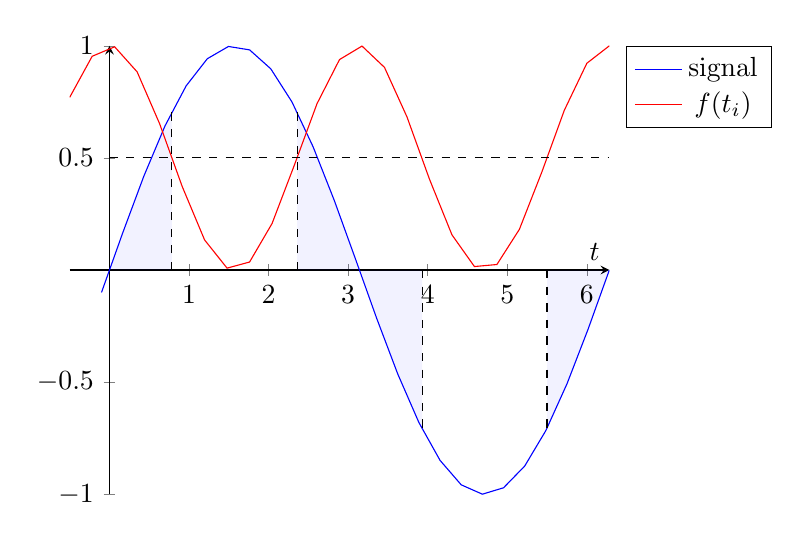
\begin{tikzpicture}
	\begin{axis}[axis lines=center, xlabel=$t$, domain=-.5:2*pi, legend pos=outer north east]
	\addplot[color=blue, name path=signal, domain=-.1:2*pi] {sin(deg(x))}; \addlegendentry{signal}
	\addplot[color=red] {cos(deg(x))^2}; \addlegendentry{$f(t_i)$}
	\addplot[mark=none,dashed, domain=0:2*pi]{.5};
	\draw[dashed] (axis cs:.785,0) -- (axis cs:.785,{sin(deg(.785))});
	\draw[dashed] (axis cs:2.36,0) -- (axis cs:2.36,{sin(deg(2.36))});
	\draw[dashed] (axis cs:3.93,0) -- (axis cs:3.93,{sin(deg(3.93))});
	\draw[dashed] (axis cs:5.5,0) -- (axis cs:5.5,{sin(deg(5.5))});
	\path[name path=axis] (axis cs:0,0) -- (axis cs:2*pi,0);
	\addplot[fill=blue, opacity=.05] fill between [of=signal and axis, soft clip={domain=0:.785}];
	\addplot[fill=blue, opacity=.05] fill between [of=signal and axis, soft clip={domain=2.36:3.93}];
	\addplot[fill=blue, opacity=.05] fill between [of=signal and axis, soft clip={domain=5.5:2*pi}];
	\end{axis}     
	\end{tikzpicture}
	
\end{document}